\def \imgpath {"./figures/lhc"}

\section{European Organisation for Nuclear Research}
CERN, located near Geneva, Switzerland, is an esteemed scientific institution dedicated to the study of particle physics, nuclear physics, and related fields. Established in 1954 by a consortium of European countries, it currently has 23 member states and collaborates with over 50 countries worldwide. Its research endeavors focus on advancing our understanding of the fundamental particles and forces that govern them.

One of the most significant and celebrated discoveries made by CERN is the Higgs boson, a particle that confers mass to other particles and is a crucial component of the Standard Model of particle physics. This discovery was made in 2012 by the ATLAS and CMS experiments, two of the four main experiments at CERN's Large Hadron Collider (LHC), the world's largest and most powerful particle accelerator.

Apart from the LHC, CERN houses several research facilities, including the Proton Synchrotron and the Super Proton Synchrotron, that provide beams of particles for a wide range of experiments. %In sum, CERN is a preeminent international center for pioneering research in particle physics and allied domains, and its findings and technological advancements have contributed substantially to our understanding of the universe. Furthermore, it embodies the potency of international collaboration and cooperation in scientific exploration.

\section{Large Hadron Collider (LHC)}

The Large Hadron Collider (LHC) is a particle accelerator that utilizes a circular tunnel with a circumference of 27 kilometers to accelerate beams of protons or heavy ions to high energies and collide them at four separate experimental locations. The LHC operates on the principle of accelerating these beams to nearly the speed of light through a series of superconducting magnets and then directing them to collide with each other at specific points along the circular path.

The LHC's superconducting magnets are cooled to temperatures close to absolute zero (-271.3 degrees Celsius) to maintain their superconducting state, allowing them to guide and focus the particle beams as they travel along the circular path. These magnets produce a strong magnetic field that keeps the particle beams on their circular trajectory and causes them to bend as they pass through the magnetic field. By adjusting the strength of the magnetic field, the LHC can control the curvature of the particle beams and ensure that they collide at the designated interaction points.

The LHC's acceleration process occurs in a series of stages, starting with a source of particles that are injected into a linear accelerator (LINAC). The LINAC accelerates the particles to an energy of a few million electronvolts (MeV) before passing them to a circular accelerator called a Booster. The Booster further accelerates the particles to an energy of 1.4 billion electronvolts (GeV) before injecting them into the Proton Synchrotron (PS).

The PS is a circular accelerator that increases the energy of the particles to 25 GeV before injecting them into the Super Proton Synchrotron (SPS). The SPS is a larger circular accelerator that further accelerates the particles to 450 GeV before finally injecting them into the LHC. Once inside the LHC, the particles are accelerated to their final energy and directed to collide at the designated interaction points.

The collisions at the LHC produce a shower of subatomic particles that are captured and analyzed by the LHC's four primary detectors: ATLAS, CMS, LHCb, and ALICE. These detectors are designed to measure the properties and trajectories of the particles produced by the collisions and provide valuable insights into the fundamental nature of matter and the universe.

Overall, the operational principle of the LHC is based on the precise control of the particle beams through a series of superconducting magnets and accelerators to produce high-energy collisions that enable cutting-edge research in particle physics.

The LHC tunnel is situated approximately 100 meters underground, in a tunnel that was previously used by the Large Electron-Positron Collider (LEP). It has a diameter of 3.8 meters and houses over 1,600 superconducting magnets. The collider operates for periods of several months at a time, with periods of downtime in between for maintenance and upgrades.

TBA Luminosity, bunches, Van der Meer scans

\begin{figure}%[!h]
\centering%
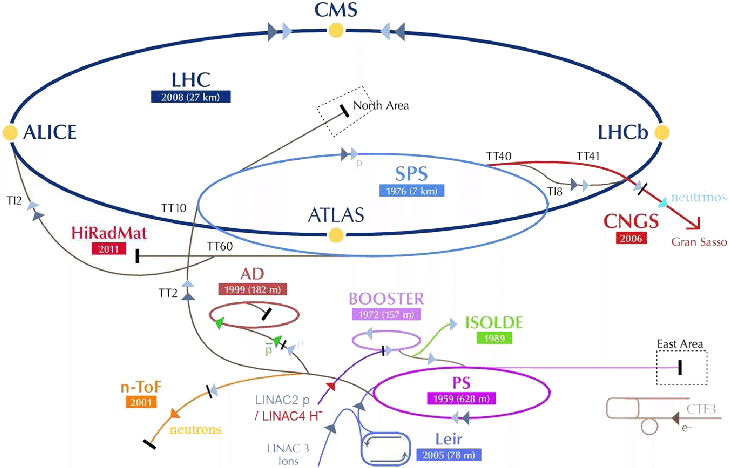
\includegraphics[width=.7\textwidth]{\imgpath/cern.png}
\caption{TBA.}
\label{fig:experiment:cern}
\end{figure}


\begin{figure}%[!h]
\centering%
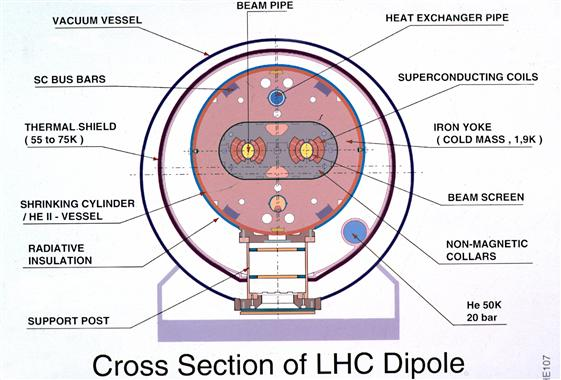
\includegraphics[width=.7\textwidth]{\imgpath/dipole.jpg}
\caption{TBA.}
\label{fig:experiment:cern}
\end{figure}